\section{自治系统稳定性的概念}\label{2Aref}
考虑自治系统的自由运动
\begin{equation}\label{freeofauto}
  \dot{x}=f(x)
\end{equation}
其中$f:D\to\R{}^n$是从$D$至$\R{}^n$的局部Lipschitz映射,$D\subset\R{}^n$为包含$x=0$的域,这保证了上式的解存在且唯一。假定$f(0)=0$,意即$x=0$为一平衡点。根据上章末尾的讨论,不妨设初始时刻$t_0=0$。
\begin{note}
  对于自治系统而言,假定$x=0$为平衡点并不失去一般性。因为若考虑一非零平衡点$x^\ast$,意即其满足$f(x^\ast)=0$,那么作变换$z=x-x^\ast$,即有\[\dot{z}=\dot{x}=f(x)=f(z+x^\ast)\]令$g(z)=f(z+x^\ast)$,则\[g(z)=0\implies f(z+x^\ast)=0\implies z=0\]因此$x^\ast$的稳定性问题同样可归于讨论$z=0$的稳定性问题。
\end{note}
\begin{definition}[自治系统的稳定性]
  式 \eqref{freeofauto} 的平衡点$x=0$是
  \begin{itemize}[leftmargin=1em]
    \item {\bf 稳定的(stable)}\index{稳定的(stable)},若对于任意$\varepsilon>0$,均存在$\delta=\delta(\varepsilon)>0$(意即,存在与$\varepsilon$有关的$\delta$),使得
    \[\|x(0)\|<\delta\implies \|x(t)\|<\varepsilon,\forall t\ge 0\]
    \item {\bf 不稳定的(unstable)}\index{不稳定的(unstable)},若其不是稳定的;意即,对于某个$\varepsilon>0$,不存在$\delta>0$使得第一点中的式子成立。
    \item {\bf 渐近稳定的(asymptotically stable)}\index{稳定的(stable)!渐近$\sim$(asymptotically)},若其稳定且存在$c>0$使得\[\|x(0)\|<c\implies \lim_{t\to\infty}x(t)=0\]
    \item {\bf 指数稳定的(exponentially stable)}\index{稳定的(stable)!指数$\sim$(exponentially)},若存在两个实数$\alpha,\lambda>0$使得\[\|x(0)\|<\delta\implies \|x(t)\|<\alpha\|x(0)\|\mathrm{e}^{-\lambda t},\forall t\ge 0\]
    \item {\bf 临界稳定的(marginally stable)}\index{稳定的(stable)!临界$\sim$(marginally)},若$x=0$是稳定的,但不是渐近稳定的。
    \item {\bf 全局渐近稳定/指数稳定的(globally asymptotically/exponentially stable)},若上述渐近稳定或指数稳定对于任意初始状态都成立。
  \end{itemize}
\end{definition}

\begin{note}
  指数稳定表明$x(t)$以较一指数函数更快的速率随$t\to\infty$而趋于$0$。一般而言,指数稳定蕴涵渐近稳定。对于线性系统而言,指数稳定和渐近稳定是等价的。
\end{note}
下面以图示说明稳定性与不稳定性。前三例来自前言中参考文献2第49-51页,最后一例来自参考文献3第12-13页。
\newpage
\begin{example}[稳定与不稳定的图示]\label{stable_unstable}
  \begin{itemize}[leftmargin=1em]
    \item 下图展示了不同稳定情况的状态轨线的运动。稳定的曲线1、2对于$\|x(t)\|<R$的情况能在某个以$r$为半径的球域$S_r$内找到一个$x(0)$作为初始,且渐近稳定的曲线1的状态还会随$t\to\infty$而趋于$0$,临界稳定的曲线2不会趋于$0$;而对于不稳定的曲线3,则可以找到一半径为$R$的球域$S_R$,使得起始状态无论距离原点多近(或者说,无论初始状态所属的球域$S_r$半径多小),解总会超出$S_R$。
    \begin{center}
      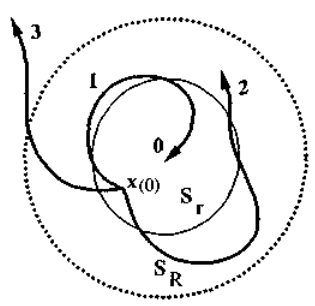
\includegraphics[width=0.3\linewidth]{figure/nonlinear/stable.png}
      \captionof{figure}{稳定与不稳定的示例}
    \end{center}
    \item 考虑如下范德坡(Van der Pol)方程\[\begin{cases}
      \dot{x}_{1}=x_{2}\\\dot{x}_{2}=- x_{1}+(1-{x_{1}}^{2})x_{2}
    \end{cases}\]
    原点是其平衡点。绘出其相轨迹,发现自任意非零状态出发的状态均会趋于一{\bf 极限环(limit cycle)}。\index{极限环(limit cycle)}因此,在极限环内任取一球域,则可见自任意接近原点(也即起始状态的球域半径任意小)的状态出发的轨线最终均会超出该球域而到达极限环,则原点不稳定。此例说明,对于非线性系统,不稳定的形式有多种,未必是线性系统中更常见的“发散至无穷远处”。
    \begin{center}
      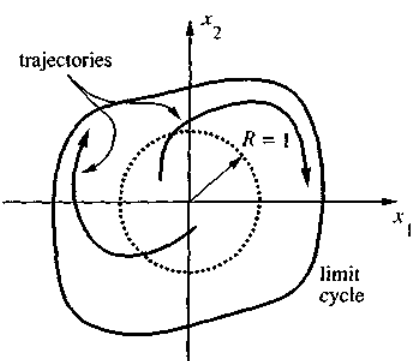
\includegraphics[width=0.34\linewidth]{figure/nonlinear/vanderpol.png}
      \captionof{figure}{范德坡方程的相轨迹}
    \end{center}
    \item 在下图所示的系统中,所有自单位球内非零初始状态出发的轨线,均会先向外到达$C$后再收敛回原点。因此,起始状态无论距离原点多近,解总会超出单位球域,即原点是不稳定的。然而,当时间足够长时,从单位球域内出发的状态总会趋于$0$,即收敛于原点。这也是在渐近稳定性的定义中需要首先以稳定为前提的原因。{\it 称这种轨迹不稳定是合理的,因为类似图中$C$这样的曲线可能已经位于模型可用范围之外。例如,飞机在亚音速和超音速情形下的动力学完全不同。假若我们按亚音速动力学模型绘制出下面相图,那么$C$可能已经进入超音速区域,那么达到$C$的轨线就不再可用。}
    \begin{center}
      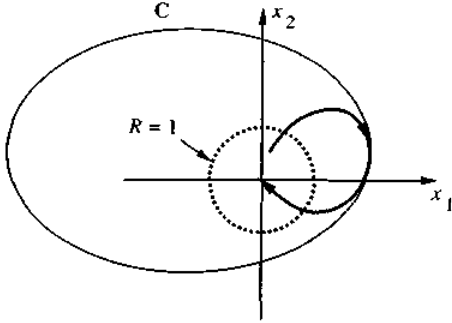
\includegraphics[width=0.35\linewidth]{figure/nonlinear/unstable.png}
      \captionof{figure}{具有收敛性但不稳定的例子之一}
    \end{center}
    \item 考虑系统方程\[\begin{cases}
      \dot{x}=f(x)+y\\\dot{y}=-x
    \end{cases}\]
    其中\[
      f(x)=\begin{cases}-4x,&x>0\\2x,&-1\le x\le 0\\-x-3,&x<-1
    \end{cases}\]
    可分三段求出系统的通解为
    \begin{align*}
      &\begin{cases}x=C_{1}(2-\sqrt{3})\mathrm{e}^{(-2+\sqrt{3})t}+C_{2}(2+\sqrt{3})\mathrm{e}^{(-2-\sqrt{3})t}\\
        y=C_{1}\mathrm{e}^{(-2+\sqrt{3})t}+C_{2}\mathrm{e}^{(-2-\sqrt{3})t}\end{cases}&(x>0)\\
      &\begin{cases}x=C_{1}\mathrm{e}^{t}+C_{2}t\mathrm{e}^{t}\\
        y=(-C_{1}+C_2)\mathrm{e}^{t}-C_{2}t\mathrm{e}^{t}\end{cases}&(-1\le x\le 0)\\
      &\begin{cases}x=\frac{1}{2}\mathrm{e}^{-\frac{t}{2}} C_{1}\Big(\cos\frac{\sqrt{3}}{2}t + \sqrt{3} \sin\frac{\sqrt{3}}{2}t\Big)
        +\frac12\mathrm{e}^{-\frac t2} C_2\Big(\sin\frac{\sqrt{3}}2t-\sqrt{3}\cos\frac{\sqrt{3}}2t\Big) \\
        y=C_{1}\mathrm{e}^{-\frac{t}{2}}\mathrm{cos}\frac{\sqrt{3}}{2}t+C_{2}\mathrm{e}^{-\frac{t}{2}}\mathrm{sin}\frac{\sqrt{3}}{2}t+3 \end{cases}&(x<-1)
    \end{align*}
    根据上面的解绘制出相轨迹如下,可知此系统不稳定,但所有解均会趋于原点。
    \begin{center}
      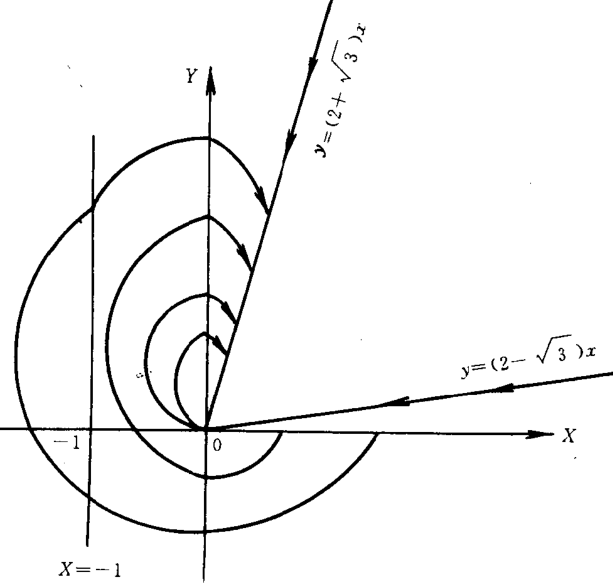
\includegraphics[width=0.4\linewidth]{figure/nonlinear/unstable2.png}
      \captionof{figure}{具有收敛性但不稳定的例子之二}
    \end{center}
  \end{itemize}
\end{example}

\begin{example}[稳定与不稳定的计算例]
  以下两例中$x=0$均为平衡点。\begin{itemize}[leftmargin=1em]
    \item 考虑方程$$\dot{x}=-(1+\sin^2x)x$$
其解为$x(t)=x(0)\mathrm{e}^{-\int_{0}^{t}(1+\sin^{2}\tau)\diff\tau}\Rightarrow\|x(t)\|\leq\|x(0)\|\mathrm{e}^{-t}.$
因此,状态$x$指数收敛至$x=0$(其中$\lambda=1$)。
\item 考虑方程$$\dot{x}=-x^2,x(0)=1$$
其解为 $x(t)=\frac1{t+1}$,则$x=0$为渐近稳定的,但不是指数稳定的。
  \end{itemize}
\end{example}
